% Copyright (C) 2014-2017 by Thomas Auzinger <thomas@auzinger.name>

\documentclass[draft,final]{vutinfth} % Remove option 'final' to obtain debug information.

% Load packages to allow in- and output of non-ASCII characters.
\usepackage{lmodern}        % Use an extension of the original Computer Modern font to minimize the use of bitmapped letters.
\usepackage[T1]{fontenc}    % Determines font encoding of the output. Font packages have to be included before this line.
\usepackage[utf8]{inputenc} % Determines encoding of the input. All input files have to use UTF8 encoding.

% Extended LaTeX functionality is enables by including packages with \usepackage{...}.
\usepackage{amsmath}    % Extended typesetting of mathematical expression.
\usepackage{amssymb}    % Provides a multitude of mathematical symbols.
\usepackage{mathtools}  % Further extensions of mathematical typesetting.
\usepackage{microtype}  % Small-scale typographic enhancements.
\usepackage{paralist} %Allows usage of inline lists
\usepackage[inline]{enumitem} % User control over the layout of lists (itemize, enumerate, description).
\usepackage{multirow}   % Allows table elements to span several rows.
\usepackage{booktabs}   % Improves the typesettings of tables.
\usepackage{subcaption} % Allows the use of subfigures and enables their referencing.
%\usepackage[ruled,linesnumbered,algochapter]{algorithm2e} % Enables the writing of pseudo code.
\usepackage{algorithm} %For algorithms
\usepackage[noend]{algpseudocode}%Allows pseudo-code like syntax in algorithms
\usepackage{tabularx}
\usepackage[usenames,dvipsnames,table]{xcolor} % Allows the definition and use of colors. This package has to be included before tikz.
\usepackage{nag}       % Issues warnings when best practices in writing LaTeX documents are violated.
\usepackage{todonotes} % Provides tooltip-like todo notes.
\usepackage{hyperref}  % Enables cross linking in the electronic document version. This package has to be included second to last.
\usepackage[acronym,toc]{glossaries} % Enables the generation of glossaries and lists fo acronyms. This package has to be included last.
\usepackage[babel=true]{csquotes} %Just more quote handling


% Define convenience functions to use the author name and the thesis title in the PDF document properties.
\newcommand{\authorname}{Stefan Gamerith} % The author name without titles.
\newcommand{\thesistitle}{Context Enrichment of Crowdsourcing Tasks for Ontology Validation} % The title of the thesis. The English version should be used, if it exists.

% Set PDF document properties
\hypersetup{
    pdfpagelayout   = TwoPageRight,           % How the document is shown in PDF viewers (optional).
    linkbordercolor = {Melon},                % The color of the borders of boxes around crosslinks (optional).
    pdfauthor       = {\authorname},          % The author's name in the document properties (optional).
    pdftitle        = {\thesistitle},         % The document's title in the document properties (optional).
    pdfsubject      = {Subject},              % The document's subject in the document properties (optional).
    pdfkeywords     = {a, list, of, keywords} % The document's keywords in the document properties (optional).
}

\setpnumwidth{2.5em}        % Avoid overfull hboxes in the table of contents (see memoir manual).
\setsecnumdepth{subsection} % Enumerate subsections.

\nonzeroparskip             % Create space between paragraphs (optional).
\setlength{\parindent}{0pt} % Remove paragraph identation (optional).

\makeindex      % Use an optional index.
\makeglossaries % Use an optional glossary.
%\glstocfalse   % Remove the glossaries from the table of contents.

% Set persons with 4 arguments:
%  {title before name}{name}{title after name}{gender}
%  where both titles are optional (i.e. can be given as empty brackets {}).
\setauthor{}{\authorname}{BSc.}{male}
\setadvisor{}{Reka Marta Sabou}{MSc., PhD}{female}

% For bachelor and master theses:
%\setfirstassistant{Pretitle}{Forename Surname}{Posttitle}{male}
%\setsecondassistant{Pretitle}{Forename Surname}{Posttitle}{male}
%\setthirdassistant{Pretitle}{Forename Surname}{Posttitle}{male}

% For dissertations:
%\setfirstreviewer{Pretitle}{Forename Surname}{Posttitle}{male}
%\setsecondreviewer{Pretitle}{Forename Surname}{Posttitle}{male}

% For dissertations at the PhD School and optionally for dissertations:
% \setsecondadvisor{Pretitle}{Forename Surname}{Posttitle}{male} % Comment to remove.

% Required data.
\setaddress{Linzerstrasse 429/4215, 1140 Wien}
\setregnumber{0925081}
\setdate{01}{01}{2001} % Set date with 3 arguments: {day}{month}{year}.
\settitle{\thesistitle}{\thesistitle} % Sets English and German version of the title (both can be English or German). If your title contains commas, enclose it with additional curvy brackets (i.e., {{your title}}) or define it as a macro as done with \thesistitle.
%\setsubtitle{Optional Subtitle of the Thesis}{Optionaler Untertitel der Arbeit} % Sets English and German version of the subtitle (both can be English or German).

% Select the thesis type: bachelor / master / doctor / phd-school.
% Bachelor:
%\setthesis{bachelor}
%
% Master:
\setthesis{master}
\setmasterdegree{dipl.} % dipl. / rer.nat. / rer.soc.oec. / master
%
% Doctor:
%\setthesis{doctor}
%\setdoctordegree{rer.soc.oec.}% rer.nat. / techn. / rer.soc.oec.
%
% Doctor at the PhD School
%\setthesis{phd-school} % Deactivate non-English title pages (see below)

% For bachelor and master:
\setcurriculum{Software Engineering / Internet Computing}{Software Engineering / Internet Computing} % Sets the English and German name of the curriculum.

% For dissertations at the PhD School:
%\setfirstreviewerdata{Affiliation, Country}
%\setsecondreviewerdata{Affiliation, Country}


\begin{document}

\frontmatter % Switches to roman numbering.
% The structure of the thesis has to conform to
%  http://www.informatik.tuwien.ac.at/dekanat

\addtitlepage{naustrian} % German title page (not for dissertations at the PhD School).
\addtitlepage{english} % English title page.
\addstatementpage

\begin{danksagung*}
\todo{Ihr Text hier.}
\end{danksagung*}

\begin{acknowledgements*}
\todo{Enter your text here.}
\end{acknowledgements*}

\begin{kurzfassung}
\todo{Ihr Text hier.}
\end{kurzfassung}

\begin{abstract}
\todo{Enter your text here.}
\end{abstract}

% Select the language of the thesis, e.g., english or naustrian.
\selectlanguage{english}

% Add a table of contents (toc).
\tableofcontents % Starred version, i.e., \tableofcontents*, removes the self-entry.

% Switch to arabic numbering and start the enumeration of chapters in the table of content.
\mainmatter



\chapter{Introduction}
\todo{Enter your text here.}
\section{Motivation}
\todo{Enter your text here.}
\section{Aim of the Work (e.g. Research Questions)}
\todo{Enter your text here.}
\section{Contributions}
\todo{Enter your text here.}
\section{Structure of the Work}
\todo{Enter your text here.}



\chapter{State of the Art}
\todo{Enter your text here.}
\section{Crowdsourcing}
\todo{Enter your text here.}
\section{Crowdsourcing in the Semantic Web}
\todo{Enter your text here.}
\section{The uComp Protege Plugin}
\todo{Enter your text here.}
\section{Enrichment of crowdsourcing tasks with contextual data}
\todo{Enter your text here.}



\chapter{Methodology}
\todo{Enter your text here.}



\chapter{Context Enrichment Methods}\label{chap:context_enrichment_methods}
While in~\hyperref[chap:implementation]{Chapter~\ref*{chap:implementation}} the technical foundation for implementing the Context Enrichment Methods was built, this Chapter describes these on a more conceptual level. There was no limitation on the used settings or data. Instead, the context used for ontology validation was created from general purpose internal and external sources. 

First, \hyperref[sec:neighboring_nodes]{Section~\ref*{sec:neighboring_nodes}} introduces a novel Context Enrichment Method which takes neighboring nodes~(i.e. subclass relations) into account. Second, a method of embedded context using metadata is discussed in \hyperref[sec:embedded_context]{Section~\ref*{sec:embedded_context}} and last, \hyperref[sec:external_source]{Section~\ref*{sec:external_source}} contains Context Enrichment using data from external sources.
\section{Neighboring Nodes}\label{sec:neighboring_nodes}
This Section starts with an conceptual overview of how neighboring nodes in an ontology graph are used to generate contextual information for ontology validation. Then, existing approaches on generating textual definitions for an ontology are examined. As in the literature~\cite{soton265735} the term \textit{ontology verbalisation} is commonly used as a short-term for that task, it is used in the remainder of this Section. We conclude that even though that there exists the major tool \textit{OWL Verbalizer}\footnote{\url{http://mcs.open.ac.uk/nlg/SWAT/Verbaliser.html} accessed 2018/04/30} which transforms a generic OWL~ontology into english sentences, we could not integrate it into Context Enrichment process because 
\begin{inparaenum}[a)]
		\item it was designed as a standalone tool written in SWI-Prolog\footnote{\url{http://www.swi-prolog.org/} accessed 2018/04/30} and
		\item as input it only accepts the whole OWL~ontology 
\end{inparaenum}.
However, to make concept definitions and relations more understandable for non-experts, some revised rules were integrated in our enrichment process.

To illustrate the concept of neighboring nodes and how they relate to the Context Enrichment approach explained later, a simple ontology graph is given in~\hyperref[fig:simple_owl_graph]{Figure~\ref*{fig:simple_owl_graph}} describing the teacher/pupil domain.
\begin{figure}
	 \centering
	 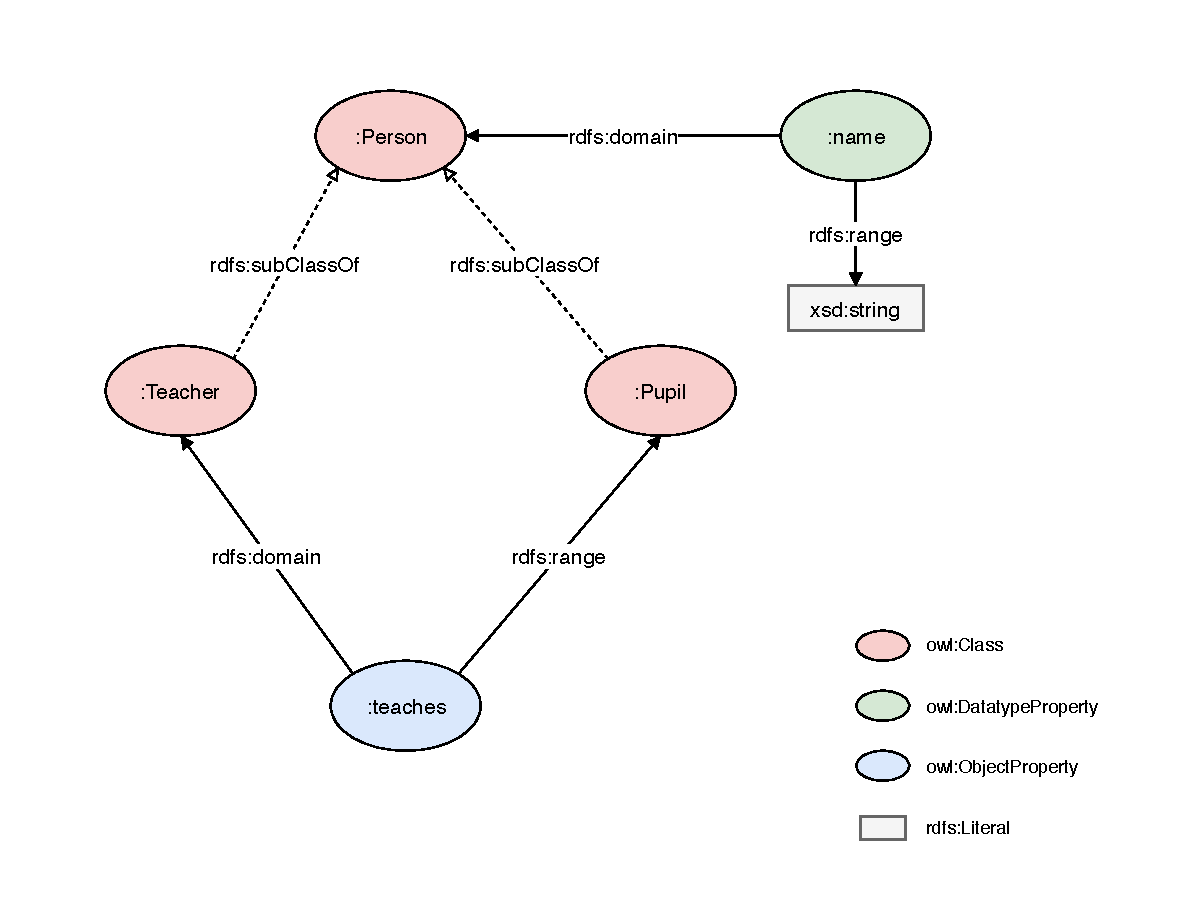
\includegraphics[width=\textwidth]{drawio/University_Ontology_Example}
	 \caption{Simple OWL ontology graph}\label{fig:simple_owl_graph}
\end{figure}
For example, if the concept \textit{:Teacher} is taken as reference node, it makes sense to not only consider the concept itself, but instead include connected nodes~(e.g. the concept \textit{:Person} and the object property \textit{:teaches}) in the enrichment process. 

As in the guidelines for conducting crowdsourcing research~\cite{sarasua2015crowdsourcing}, the authors recommended to avoid technical terms in crowdsourcing questions. To facilitate this need, we examined an existing approach on ontology verbalisation and how they could be integrated in the Context Enrichment process. 

Despite the fact that natural language is desirable for descriptions as everybody knows and understands it with no extra learning effort, it conflicts with highly expressive, domain specific and formal knowledge representations. Formally specified ontologies on the other hand facilitate encoding complex relations in domain-specific areas. To resolve this conflict, the new language variant \textbf{ACE}~\textit{(Attempto Controlled English)}~\cite{fuchs2008} was proposed. ACE is a formal language, capable of expressing domain-specific knowledge with a well-defined syntax, supporting formal reasoning and readable by specialists who are yet unfamiliar with formal languages and methods.

As our approach described later in this section is based on ACE\footnote{\url{https://tinyurl.com/yc3zhu9a} accessed 2018/05/05}\footnote{\url{https://tinyurl.com/ycst39jv} accessed 2018/05/05}, a short overview of ACE' language structure is given in the following paragraphs:
 
 \paragraph{Simple Sentences} A Simple Sentence derived from standard English contains a subject and a verb: \texttt{subject + verb + complements [ + adjuncts ]} In addition the verb relate direct or indirect to one or more other objects~(\textit{complements}). Optionally, to add more specificity one or more adverbs and prepositional phrases can be added~(\textit{adjuncts}). 

\paragraph{Composite Sentences} A Composite Sentence is recursively built from one or more Simple Sentences connected by \textit{coordination},
\textit{subordination}, \textit{quantification} and \textit{negation}. Whereas, coordination is associates sentences either by the word \texttt{and} or \texttt{or}, subordination describes dependent sentences in some form of relation to each other~(e.g. if-then sentences). Quantification enables expressing statements about all~(universal quantification) or certain~(existential quantification) objects of a certain domain. Last, negation is a way encode negative polarity in a sentence~(e.g. sentences containing \texttt{not} or \texttt{no}). 

\paragraph{Query Sentences} Query Sentences can be divided into polar questions~(e.g. with \textit{yes/no} answer) and non-polar questions, also known as \emph{wh-questions}. For those there does not exist a pre-defined answer, as in contrast to the former yes/no questions. Furthermore, wh-questions start with either of the following five W-words: \texttt{Who}, \texttt{What}, \texttt{When}, \texttt{Where} and \texttt{Why}. However, sometimes questions starting with the word \texttt{How} are added to the category of wh-questions.

\paragraph{Anaphoric References} In case the meaning of a word or phrase depends on the context, multiple occurrences of these expressions are called \textit{Anaphoric References}. More specifically, the referring term~(\textit{anaphor}) relates to an antecedent expression. For example in the sentence \texttt{Tom arrived, but nobody noticed him}, the pronoun \texttt{him} relates to \texttt{Tom}. To resolve ambiguities during the processing phase, Anaphoric References are replaced by encoded references. 

Among others, one application areas of ACE is \textbf{OWL Verbalizer}~\cite{stevens2011}, an open source tool aiming at producing ACE texts from generic OWL ontologies. A description on the major concepts of OWL Verbaliser where our approach is based on is given below:

To overcome the burden of manual authoring ontology definitions, the tool formally known as OWL Verbaliser and now part of the \textbf{SWAT Tool Suite}\footnote{\url{http://mcs.open.ac.uk/nlg/SWAT/} accessed 2018/05/06} was created. Whereas producing high quality texts in restricted application domains is an active research field, this tool aims at generating understandable und useful descriptions that are of moderate quality using general-purpose methods.

The high-level process of ontology verbalization depicted from \hyperref[fig:verbaliser_architecture]{Figure~\ref*{fig:verbaliser_architecture}} consists of the following stages:

\paragraph{Transcoding from OWL to Prolog} Using an ontology in RDF/XML~Format as input, a file in a convenient Prolog format is generated in this
stage. The conversation process covered by the \textit{Transcoder}, \textit{Identifier~Selector} and \textit{Label~Selector} groups identifiers~(concepts, individuals, object~properties) together with labels for further processing. In addition, ambiguous terms in identifiers are standardised. 

\paragraph{Constructing a lexicon for atomic entities} The output of this stage, covered by the component \textit{Lexicon Generator}, is a collection of lexicons, computed from the normalised Prolog terms in the previous stage. A lexical entry~(lexicon) is defined as a quadruple of the following form: \texttt{<identifier, part-of-speech, singular-form, plural-form>} To facilitate processing in later stages, normalised identifiers for concepts, individuals and object~properties processed in the beginning are stored together with word category, singular form and plural form. The word~category, in linguistics also known as part-of-speech, groups words based on similar properties in terms of syntax and grammar. Common categories among others are nouns, verbs and adjectives. Last, to differentiate the quantity of described by a phrase or word, the singular and plural form of a noun is associated with each lexical entry. 
Among the storage of lexicons, the algorithm has some further rules concerning text processing implemented.  Some simple heuristics are used for pre-processing to transform the resulting word string into better readable English phrases. 

\paragraph{Selecting the axioms relevant for describing each class} This stage and next stage are covered by the \textit{Planner}.
This component has as input all axioms from the source ontology as well as the lexicons from the previous stage. In this stage axioms associated with matching lexical entries. The algorithm uses the identifier in the lexicon and the IRI~\cite{rfc3987} in ontological elements as matching criteria. 

\paragraph{Aggregating axioms with a similar structure} This stage is optional, as it is not strictly required for text generation described in the next stage. However, some improvements over using the axioms from the previous stage are achieved by grouping similar axioms. 

\paragraph{Generating sentences from axioms} The final stage is expressed by the component \textit{Realiser}, forming the central part of the
verbalisation process. English sentences are generated for each axiom using logical rules for almost every logical pattern in OWL-DL. These rules are expressed as Prolog clauses, taking the axiom and optionally the lexicon as inputs.

\begin{figure}
	 \centering
	 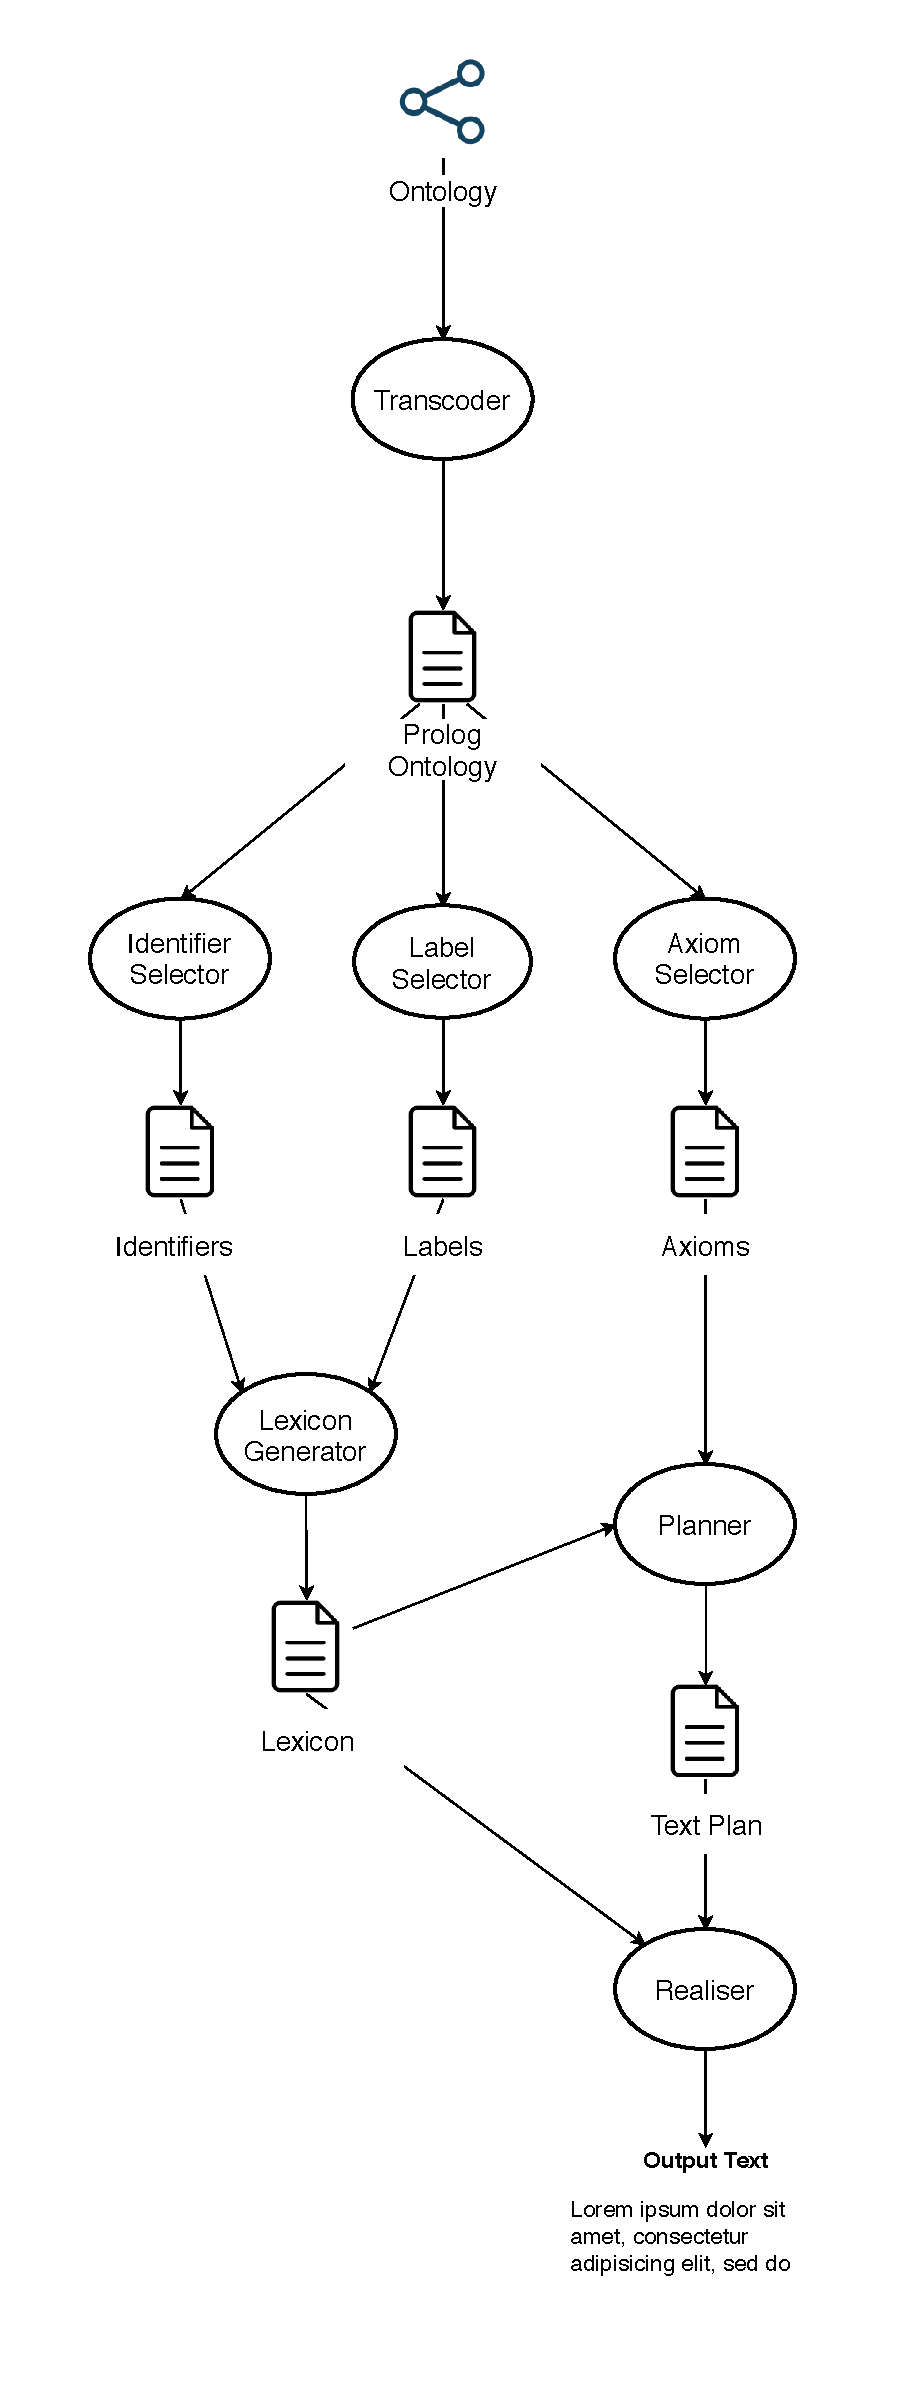
\includegraphics[width=0.5\textwidth]{drawio/Ontology_Verbaliser_Architecture}
	 \caption{Conceptual architecture of the OWL ontology verbaliser~\cite{stevens2011}}\label{fig:verbaliser_architecture}
\end{figure}

Although OWLVerbaliser would be useful to integrate in the enrichment process, there are some major differences:

The first reason is \emph{incompatibility on a language level}. Traditionally, software systems are written in many different programming languages, arising the challenge of dealing with interoperability~\cite{malone2014}. OWLVerbaliser is written in SWI-Prolog and Protege is used as the platform running on the Java Virtual Machine~(JVM), forming a conceptual mismatch in programming paradigms. Moreover, if not impossible, interoperability between conceptually different programming languages is challenging in its own\footnote{\url{http://www.swi-prolog.org/packages/jpl/} accessed 2018/05/11} and would conflict with the goal of an easily integrable solution.

Another reason is a \emph{mismatch on the operating scope}. OWLVerbaliser was implemented as a tool assisting engineers in ontology building, a process which is a time consuming manual task. It was designed as a standalone tool, launched from the command line or deployed as a web service. On the other hand ontology enrichment is embedded into Protege and part of the ontology validation process, operating only on small parts of the ontology while OWLVerbaliser takes the whole ontology as input. 

\paragraph{Proposed Approach for Ontology Validation} Due to this complicating issues, we implemented a different approach using the insights from OWLVerbaliser. The pseudocode covering the conceptual workflow is given in \hyperref[alg:neighbourhood]{Algorithm~\ref*{alg:neighbourhood}}. The notation to describe properties and relations of OWL is based on the formal Description Logic~(DL) for ontologies~\cite{baader2003} and string manipulation in formal languages~\cite{hopcroft1969}.

\begin{algorithm}
	\caption{Context Enrichment based on Neighboring Nodes}\label{alg:neighbourhood}
	\begin{algorithmic}[1]
		\Procedure{Generate Description}{}\newline
			\textbf{Input:} A concept $C$\newline
			\textbf{Output:} A textual description $T$ of $C's$ neighboring nodes based on subsumption\newline
			\State{$T=\{\}$} \label{alg:neighbourhood:text_initialisation}
			\For {$ (c,d) \in C \sqsubseteq D $}
				\State $T=T$ $\cup$ "Every " $\cup$ $name(c)$ $\cup$ " is a " $\cup$ $name(d)$
			\EndFor
			\For {$ (e,c) \in E \sqsubseteq C $}
				\State $T=T$ $\cup$ "Every " $\cup$ $name(e)$ $\cup$ " is a " $\cup$ $name(c)$
			\EndFor
		\EndProcedure
	\end{algorithmic}
\end{algorithm}

The main work is done in two for-loops, which calculate context descriptions based on subsumption~$(\sqsubseteq)$ and string concatenation~$(\cup)$. To handle the case of missing subsumption relations, the output text $T$ is initialised to an empty string~(\hyperref[alg:neighbourhood:text_initialisation]{Line~\ref*{alg:neighbourhood:text_initialisation}}). Next, for every subsumption relation having the input concept $C$ in its signature, either $C's$ name or the anchor node's name is appended first. For example, given the following subsumption relations $\{Car \sqsubseteq Vehicle, Cabrio \sqsubseteq Car\}$, the algorithm generates $T=\{$\textit{"Every Car is a Vehicle"}$,$ \textit{"Every Cabrio is a Car"}$\}$ under the assumption that \textit{Car} was chosen as reference node.  

\section{Embedded Context}\label{sec:embedded_context}
Over the years several ontologies covering a wide area of application have emerged, including general-purpose as well as highly specialised ones. It is evident that one of the most important aspects is their content. In addition, a key characteristic among others~\cite{daquin2012} of a good ontology is its documentation. To get an overview of existing approaches several ontologies were analysed~\cite{dutta2017}. The outcome was that there is no standard way to describe and document ontologies. However, some vocabularies with embedded descriptions were present. 

In this Section we give an overview of existing approaches for embedding metadata in ontologies and explain the approach we integrated in the validation process in detail. In the remainder of this Section our focus lies on metadata vocabularies in the context of ontology engineering. A broader discussion on the use of metadata in general is given in~\cite{nilsson2010}. 

\paragraph{Dublin Core~(DC)} Being one of the most prominent vocabulary in describing metadata, published and maintained by the Dublin Core Metadata Initiative~(DCMI), it originally contained 15 metadata terms\footnote{\url{http://www.dublincore.org/documents/dces/} accessed 2018/05/20} designed to express simple textual information about resources. Since its first launch the project have gained popularity, including more than 127 terms\footnote{\url{http://www.dublincore.org/documents/dcmi-terms/} accessed 2018/05/20}. The initial set of metadata terms is listed in~\hyperref[table:dublin_core]{Table~\ref*{table:dublin_core}}. 

\begingroup
\renewcommand{\arraystretch}{2}
\begin{table}
	\begin{tabularx}{\textwidth}{l|X}
		\textbf{Name} & \textbf{Description} \\
		\hline
		\texttt{dc:contributor} & Element used to describe a person, organisation or service who is responsible for making contributions.\\
		\texttt{dc:overage} & Term used to describe a temporal topic~(e.g. period, date, or date range), spatial topic~(e.g. location or place identified by its name or coordnates) or a jurisdiction~(e.g. an administrative entity). \\
		\texttt{dc:creator} & A person, organisation or service who created this entity.\\
		\texttt{dc:date} & A period or point in time associated with an event in the lifecycle.\\
		\texttt{dc:description} & A natural-language definition.\\
		\texttt{dc:format} & Defines the file format, physical medium or dimension.\\
		\texttt{dc:identifier} & A unique and unambiguous reference to this entity within a defined context.\\
		\texttt{dc:language} & The language used to describe and define this entity.\\
		\texttt{dc:publisher} & A person, organisation or service who provides access to this entity.\\
		\texttt{dc:relation} & Defines a link to another entity identified by name or formal identifier.\\
		\texttt{dc:rights} & A statement about associated rights with the entity~(e.g. intellectual property rights).\\
		\texttt{dc:source} & A related entity from which this entity is derived from.\\
		\texttt{dc:subject} & The topic of this entity represented using keywords, key-phrases or classification codes.\\
		\texttt{dc:title} & The name by which this entity is formally known.\\
		\texttt{dc:type} & Defines the genre of nature. Typically a well-defined vocabulary such as DCMI Type Vocabulary\footnote{\url{http://dublincore.org/documents/dcmi-type-vocabulary/}} is recommended here.\\
	\end{tabularx}
	\caption{The initial set of DC-Metadata terms}
	\label{table:dublin_core}
\end{table}
\endgroup

To maximize interoperability among heterogeneous application among the Web, the DCMI-Metadata elements were encoded in RDF Schema\footnote{\url{http://dublincore.org/schemas/rdfs/} accessed 2018/05/20}. Each entity is identified by a Uniform Resource Identifier~(URI) starting with \emph{http://purl.org}. 

\paragraph{Simple Knowledge Organisation~(SKOS)} The SKOS Core Vocabulary~\cite{skos2005} includes a set of RDF properties and RDFS classed used to express the content and structure a concept scheme, defined as a set of concepts optionally containing links between those concepts. The vocabulary is standardised by the W3C~Consortium\footnote{\url{https://www.w3.org/TR/skos-reference/} accessed 2018/05/20}. The most important terms related to metadata definition are listed in~\hyperref[table:skos]{Table~\ref*{table:skos}}.

\begingroup
\renewcommand{\arraystretch}{2}
\begin{table}
	\begin{tabularx}{\textwidth}{l|X}
		\textbf{Name} & \textbf{Description} \\
		\hline
		\texttt{skos:Concept} & Describes an idea, notion or unit of thought, similar to OWL classes. However the specification does draw any relations to \textit{owl:concept}.\\
		\texttt{skos:ConceptScheme} & A Concept Scheme can be viewed as a combination of multiple \textit{skos:Concept} instances with optional references to each other.\\
		\texttt{skos:altLabel} & A \textit{lexical label}~(e.g. a text composed of unicode characters) adding an alternative meaning. \\
		\texttt{skos:prefLabel} & Together with \textit{skos:altLabel} used to define the primary description if there are multiple human-readable definitions.\\
		\texttt{skos:notation} & Is a literal string of unicode characters uniquely identifying the related concept within the given concept scheme.\\
		\texttt{skos:changeNote} & Belongs to the class of \textit{documentation properties} and provides some information about historical changes.\\
		\texttt{skos:definition} & Adds a human readable definition text.\\
		\texttt{skos:note} & Some arbitrary text which may be provided by ontology engineers.\\
		\texttt{skos:editorialNote} & A note added by creators to inform ontology maintainers.\\
		\texttt{skos:historyNote} & A historical note~(e.g. a version string, release date, \ldots )\\
        \texttt{skos:related} & Indicates that SKOS concepts are somewhat related to each other.\\
	\end{tabularx}
	\caption{A subset of the SKOS vocabulary}
	\label{table:skos}
\end{table}
\endgroup

There is some overlap between DC and SKOS. For example, the term \textit{dc:subject} describes similar characteristics of an entity as the property \textit{skos:subject}. However, in some usage scenarios the range of the latter is restricted to resources of type skos:concept whereas the former is completely unrestricted. Moreover, in case there exists more than one subjects, the property \textit{skos:primarySubject} allows asserting the main subject of an entity or resource. 

\paragraph{Open Biomedical Ontology~(OBO)} Biological systems traditionally a complex field with increasing data sets require well defined interfaces to query, manipulate and maintain these large knowledge bases. The Open Biomedical Ontologies~(OBO)~Foundry\footnote{\url{http://obofoundry.org/} accessed 2018/05/21}, a community of ontology developers and engineers in the biomedicine domain, manage a large set of ontologies available in various formats nowadays. The most common format for biomedical ontologies is the OBO~format though, originally developed as part of the Gene Ontology~(GO)\footnote{\url{http://www.geneontology.org/} accessed 2018/05/21}. 

The OBO File Format Specification~1.2~\footnote{\url{https://owlcollab.github.io/oboformat/doc/GO.format.obo-1_2.html} accessed 2018/05/22} defines the flat document structure for OBO files. Every file is composed of a header and a multiple \emph{stanzas}. A stanza is a labeled section of the document, indicating that an object of a particular type is being described. Currently there are three supported types: \textit{Term}, \textit{Typedef} and \textit{Instance}. Every stanza starts with an id tag and an unbounded list of tag-value pairs. Studying the supported tags, it follows that the definition of metadata was important to achieve the goals of \textit{readability}, \textit{ease of parsing}, \textit{extensibility} and \textit{minimal redundancy}. In particular, it allows among others specification of 
\begin{inparaenum}[1)]
		\item the term definition (\texttt{def}),
		\item comments (\texttt{comment}),
		\item editorial data~(\texttt{is\_obsolete}, \texttt{replaced\_by}, \texttt{created\_by}, \texttt{creation\_date}) and
		\item cross references (\texttt{xref})
\end{inparaenum}.

Unfortunately the two ontology based systems the Open Biomedical Ontologies and the Semantic Web evolved independently with growing knowledge bases. To bring these two communities together, researchers have created a tool for converting OBO~ontologies to OWL and vice-versa without loosing any information during the conversion process~\cite{tirmizi2011}. It turned out that for the majority of the OBO~vocabulary the transition fits nicely into the Semantic Web Layer cake. The mapping between OBO and the Semantic Web layer cake is shown in~\hyperref[fig:semantic_obo_cake]{Figure~\ref*{fig:semantic_obo_cake}}. 

\begin{figure}
	 \centering
	 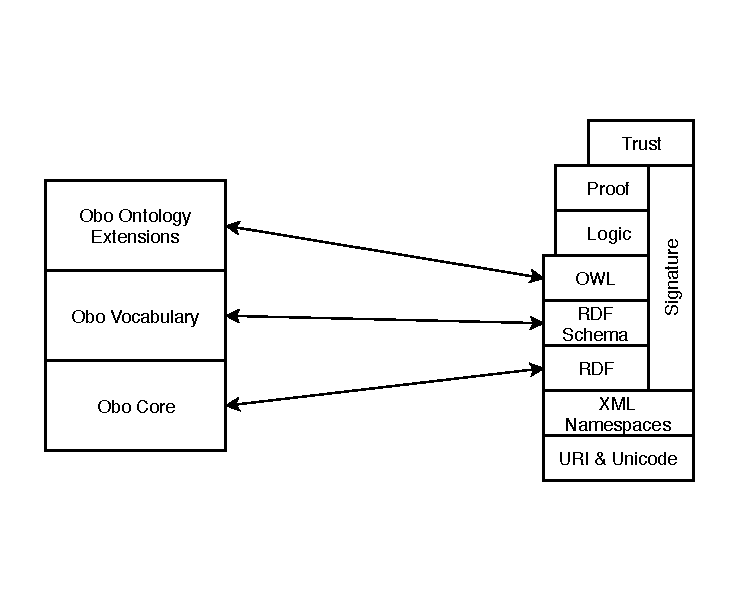
\includegraphics[width=0.5\textwidth]{drawio/Obo2Owl}
	 \caption{Mapping between the Open Biomedical Ontologies and the Semantic Web depicted from~\cite{tirmizi2011}}\label{fig:semantic_obo_cake}
\end{figure}

\emph{OBO~Core} forms the bottom layer of the OBO layer cake. It mainly handles assigning ids and namespaces to RDF related concepts. Historically OBO identifiers were limited in scope (local identifiers) while OWL requires global identifiers (URIs). This imposes some challenges on the translation process, e.g. URI need to be prepended by the scope string. 

The next layer represents the \emph{OBO Vocabulary} which is mapped to the RDF-Schema. As RDF-Schema has a replacement for each of the terms in this layer, the translation process is implemented by replacing \texttt{names} with RDFS labels, \texttt{definitions} with RDFS labels, \texttt{comments} with RDFS comments, \texttt{is\_a} with subclass relations, \texttt{domains} with RDFS domain restrictions and \texttt{ranges} with RDFS range restrictions. 

The top most layer is represented by the \emph{OBO Ontology Extensions} which are mapped to OWL. Besides the definition of concept-level mappings this layer defines tags for expressing metadata on the entire ontology. For example editorial metadata as \texttt{creation\_date}, \texttt{replaced\_by} or \texttt{saved\_by} are mapped to annotation properties. 

A summary of the most important OBO tags together with their OWL equivalents is found in~\hyperref[table:obo]{Table~\ref*{table:obo}}. Once characteristic about the mapping process resulting in some of the tags listed in the table is worth mentioning: For some of the OBO vocabulary there is on corresponding tag in the OWL vocabulary. For this reason a dedicated OWL namespace\footnote{http://www.geneontology.org/formats/oboInOwl\#} containing the definitions of all OBO specificities was created. Additionally, as OBO features are a strict subset of OWL DL, the manipulation of converted OBO features in OWL should be restricted to allow the transformation back. A more detailed discussion on this topic is given in~\cite{tirmizi2011, tirmizi2006}.

\begingroup
\renewcommand{\arraystretch}{2}
\begin{table}
	\begin{tabularx}{\textwidth}{l|l|X}
		\textbf{Name} & \textbf{OWL Translation} & \textbf{Description} \\
		\hline
        \texttt{obo:def} & oboInOwl:Definition & The definition of the term in natural language.\\
		\texttt{obo:synonym} & oboInOwl:Synonym & An indication that there exists a tag with the same meaning.\\
		\texttt{obo:comment} & rdfs:comment & A remark to the term. \\
		\texttt{obo:xref} & oboInOwl:DbXref & A reference to an analogous term in another vocabulary.\\
		\texttt{obo:date} & oboInOwl:hasDate & The creation or modification date\\
		\texttt{obo:saved-by} & oboInOwl:savedBy & The username of the person to last save this file.\\
		\texttt{obo:replaced\_by} & oboInOwl:replacedBy & A reference to a newer term which replaces this obsolete term.\\
	\end{tabularx}
	\caption{A subset of the OBO vocabulary used as metadata}
	\label{table:obo}
\end{table}
\endgroup

\paragraph{Proposed Approach for Ontology Validation} Given the various ontology metadata formats above, \hyperref[alg:embedded_enrichment]{Algorithm~\ref*{alg:embedded_enrichment}} shows the pseudocode needed to create the textual concept descriptions extracted from the embedded concept metadata. In addition to the notation from the previous Section we define $\Phi(C) \coloneqq \{m_1, m_2, \ldots, m_i \}$ where $m_i$ is the $i'th$ metadata element embedded in concept $C$, whereas $m$ represents the textual description of some metadata element.

\begin{algorithm}
	\caption{Context Enrichment based on Embedded Metadata}\label{alg:embedded_enrichment}
	\begin{algorithmic}[1]
		\Procedure{Generate Description}{}\newline
			\textbf{Input:} A concept $C$ with embedded metadata $\{m_1, m_2, \ldots, m_i \}$\newline
			\textbf{Output:} A textual description $T$ of $C's$ metadata elements\newline
			\State{$T=\{\}$}
			\For {$ m_k \in \Phi(C) $}
				\State $T=T$ $\cup$ $m_k$
			\EndFor
		\EndProcedure
	\end{algorithmic}
\end{algorithm}

While the actual enrichment is straightforward, merging just all the metadata text for a specific concept, it does not make any assumptions on how the extraction is performed because it depends on the metadata encoding. As we chose the option to encode the metadata in annotation properties, the extraction process is just a matter of selecting the appropriate annotation property for a given concept. 

\section{External Source}\label{sec:external_source}
A different method of generating textual descriptions is by concept lookup from external sources. Whereas the connected nature of a ontology is neglected, the lookup is solely based on the concept name. Dictionaries have always been the primary resource in terms of finding the information about specific words or phrases.

This Section begins with an introduction in the theory of dictionaries, discusses searching problems and strategies to overcome these, briefly introduces several online dictionaries including the one we used in our approach as external source and ends with a detailed discussion on the architecture and workflow thereof. 

\paragraph{Short Introduction to Lexicography}
Typically dictionaries include the \textit{lexicon} of a language, that is a collection of words called the lexemes, in some kind of ordered form. They facilitate the looking up of words and enable the user to find information about spelling, meaning and usage. Historically written dictionaries were constrained by the alphabetised format and once printed never updated. On the other hand their online dictionaries allows the searcher to access the information on more than on path, semantics being one of them. Similarly, keeping the word up-to-date as well as adding new ones is as simple as updating or adding new records to the database compared to printing and distributing new copies of their written counterparts. 

Lexicography is the science about~\enquote{the theory and practice of dictionaries, that is, dictionaries, encyclopaedias, lexica, glossaries, vocabularies, terminological knowledge bases, and other information tools covering areas of knowledge and its corresponding language.}~\cite{fuertes2017}
Among other definitions, they share the understanding that lexicography is a interdisciplinary science with characteristics of linguistic science, information science and others. 

When it comes to classifying electronic dictionaries, it is obvious that they are more than just machine-readable copies of their printed counterparts, but rather comprehensive software only limited by technological, economical and/or practical constraints. The key defining elements thereof are 
\begin{inparaenum}[i)]
		\item the access principle,
		\item the construction principle and
		\item the distinction between information databases and information tools
\end{inparaenum}~\cite{fuertes2011}.
Whereas the \textit{access principle} deals with providing quick and easy access to the needed information, the \textit{construction principle} differentiates dictionaries based on the technical and economical aspects taken into account during the initial building phase. When describing dictionaries special attention should be paid to the division between information databases and information tools, that is, separating the user concerns~(searching and viewing the results) from the underlying data organisation. 

Over the years various dictionaries serving different purposes emerged, depending on the contexts of use. A recent study~\cite{mueller_spitzer2013} evaluated how dictionaries are being used or, more formally, the external conditions or situations in which a dictionary consultation is embedded.  
Participants with professional and academic background were asked some open questions about the circumstances of dictionary usage. 

Analyses revealed that responses can be partitioned into the following \textit{groups of usage} situations: 
\begin{enumerate}
	\item Text Production
	\item Text Reception
	\item Text Translation
\end{enumerate}

\textit{Text Production} is the action of writing texts done in professional or personal context. Requirements on the content elements of a dictionary vary not only on the writers profession but also the category of the written texts matters. For example, passive speech using domain specific vocabularies are dominant in academic literature over active speech and simple language constructs in short-term, informal texts~\cite{o2010routledge}~(e.g. emails, tweets, Facebook posts, \ldots).

\textit{Text Reception} is the process or theory that emphasises the meaning and interpretation of existing literature. Readers focus on writing reviews and understanding texts, imposing different requirements on the content elements of a dictionary. The user's motivation of dictionary interaction is to find the word definition, look for samples~(e.g. example sentences), synonyms/antonyms and links to external information sources. 

\textit{Text Translation} is the process of converting text from a source language to a target language by preserving its meaning. Unfortunately there is not always a one-to-one mapping possible because of the absence of equivalent language constructs in the target language. Old-fashioned dictionaries containing exclusively consisting of word-mappings do not help either here. To introduction of online dictionaries offer new possibilities to translators as spelling correction and links to synonyms/antonyms). Not only professional translators responded that dictionaries are crucial for their business, users consider dictionary consultation to improve their vocabulary, look up pronunciation or simply find the contexts of word usage. 

\paragraph{Searching in Electronic Dictionaries} A key factor in today's electronic dictionaries is its searching capabilities. In the next few paragraphs we discuss problems that arise when searching for specific terms and strategies to overcome these. 

Several studies~\cite{pastor2010, mvechura2008} have analysed digital dictionaries, available in different languages and accessible via the Internet or compressed on a digital medium~(e.g. CD-ROM). Their evaluation is based on empirical analyses of user behaviour collected from log-files as well as literature review. The search techniques and challenges presented below tackle the problem of invalid, incomplete, misspelled and multi-word search queries.

The first category are represented by \textit{inflection-aware} search algorithms which draw the connection between inflected search search queries and its corresponding uninflected counterpart in the dictionary. The central part of these algorithms are rewrite rules which transform the input query to the matching headword in the dictionary or vice-versa. A powerful but complicated technique is based on thorough understanding of the target language by applying morphologies on the word endings. For example, whereas stripping \emph{-ed} and \emph{-ing} endings for regular verbs is yet simple and achieves good results, more sophisticated algorithms with encoded mappings of irregular verbs are needed occasionally. Another approach not taking the structure of the target language into account is matching based on fuzzy search algorithms. The well-known algorithm based on the Levenshtein~Distance~\cite{levenshtein1966} is a good candidate falling into the group of fuzzy search algorithms. 

The next category are techniques dealing with \textit{multi-word} search items. On the one hand search algorithms need to deal with user entered search strings containing multiple words or even complete sentences, whereas on the other hand dictionaries contain a multi-word entry~(e.g. phrasal verb) but users searched just for single words expecting all combinations thereof in the results. One solution for the latter challenge is to enumerate all possible combination of dictionary entries which contain the search query. While this seems applicable for dictionaries with small corpora, it is infeasible if performance is important. In these cases its is better to construct an index from the multi-word entries together with possible word combinations. An even better approach would be to preprocess the words before-hand by lemmatising.

Another challenge in processing search queries is \textit{detecting misspellings}. User input is inherently prone to errors as misspellings. Smart algorithms guide the user to the intended word by offering corrections and suggestions similar to a spellchecker. A naive approach would be to collect lists of common misspelled words and do the matching thereon. This has the disadvantage that not all possible combinations are included and processing takes longer especially for long word lists. A better but yet more complicated technique is based on word similarity. As discussed above fuzzy search algorithms are good candidates thereof. 

A technique especially useful for multi-lingual dictionaries is \textit{language selection and detection}. Due to the fact that this is a wide research area covered by many publications~\cite{mcnamee2005, lodhi2002, vatanen2010, selamat2016}, we will just discuss briefly some approaches. One group of algorithms is purely based on statistical models, trying to detect the target language by comparing the inferred statistics against the pre-trained statistics and calculating probabilistic models thereof. Another option is based on counting the common words or character sequences~(called n-grams) and comparing the obtained frequency counts against reference values~\cite{mcnamee2005}. If performance is not an issue than simultaneously searching in all sections of a multi-lingual dictionary would be the simplest solution. 

The last technique solving the problem of unwanted characters in search strings is \textit{text normalisation}. It identifies the task of removing variation and reducing text~(words) to a simpler format. For search strings, this means that noisy characters are removed using various yet simple approaches. A simple strategy is to use lists of common characters which do not add any meaning such as hyphens, dots quotation marks and (mathematical)~symbols. Inputs are then transformed by deleting all these characters and merging consecutive occurrences of whitespace. Moreover, the Unicode standard defines several variations for the same characters\footnote{\url{http://www.unicode.org/reports/tr15/} accessed 2018/06/08 } which needs to be taken into account by a normaliser. 

\paragraph{Online Dictionary Examples} We have chosen some well-known online dictionaries that were used in various research fields as evaluation
source. Their usage is free of charge, making them ideal candidates as source of reference in different use cases. 

%WordNet
Started as a research project in 1985 at Princeton University \textbf{WordNet}~\cite{fellbaum1998} is best characterised as dictionary browser rather than just online dictionary. It allows users to explore its contents on the basis of semantic, rather than alphabetic similarities. Its core principle fits better how users look up information along more than one path, semantics being among them. How one wants to explore the possibilities of online references depends rather on one's ideas as well as the applications one has in mind. 

The building blocks of WordNet are \textit{synsets} which are linked by a number of relations. A synset is defined as a set of words with similar semantics. It is important that synonymy does not entail unrestricted interchangeability. By that criterion natural languages would have very synonyms. Instead, synonymy is typically relative to a context which is modelled as links within synsets as well as to synsets as a whole. WordNet allows several classifications for these connections. Among these are \textit{polysemy/monosemy}, \textit{hyponymy/hypernymy}, \textit{meronymy/holonymy}. Whereas polysemy in contrast to its opposite monosemy describes the facts that multiple meanings for a specific word may be associated, hyponymy and its inverse hypernymy means that words or phrases are included in the meaning of another word, meronymy and its opposite holonymy denotes to a part-of or member-of relationship.

The WordNet architecture~\cite{fellbaum1998} as illustrated in~\hyperref[fig:wordnet_architecture]{Figure~\ref*{fig:wordnet_architecture}} is split into distinct parts:
\begin{enumerate}
		\item Lexical Source Files
		\item the Grinder
		\item the Lexical Database
		\item Software Tools and Interfaces
\end{enumerate}

\begin{figure}
	 \centering
	 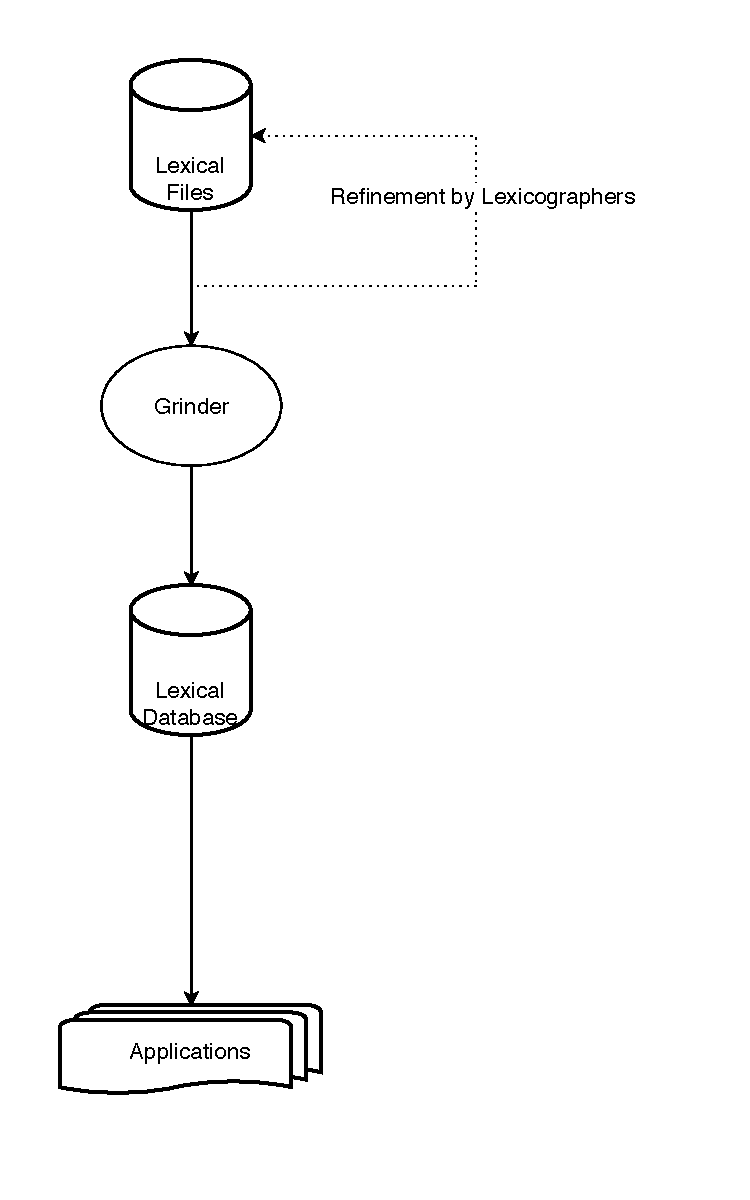
\includegraphics[width=0.5\textwidth]{drawio/WordNet_Architecture}
	 \caption{The architecture of the WordNet system~\cite{fellbaum1998}}\label{fig:wordnet_architecture}
\end{figure}

\textit{Lexical source files} are written by humans, are the result of a detailed analysis of lexical semantics and represent the set of lexical knowledge. Lexical files contain synsets from one of the following syntactic categories: nouns, verbs, adjectives and adverbs. Synonym words, relational pointers, comments and example sentences may be encoded in a synset. 

The \textit{Grinder} is a software who's main purpose is to compile the lexical source files info a database format that facilitates information querying. 
The software is implemented as a multipass compiler, similar to compilers for programming languages. In addition to database files the Grinder also generates index files used for faster information retrieval and optionally statistics of the processed synsets.  

The \textit{Lexical Database} forms the heart of the WordNet system. It is the result of a processing all lexical source files. Fortunately there are many tools to access the database. They are written in various programming languages like Perl or awk, there also exists an online query interface\footnote{\url{http://wordnetweb.princeton.edu/perl/webwn} accessed 2018/06/14}. The database uses several indexes to increase the performance of search queries, each serving a dedicated purpose. 

Users interact with WordNet with \textit{interfaces} of various forms. Different interfaces serve different purposes, depending on the area of application there are textual interfaces~(Command Line Interfaces and APIs) as well as graphical interfaces~(Desktop Software and Web Applications). 

A key success factors of WordNet is its accessibility, quality and potentials in terms of Natural Language Processing~(NLP). Various research projects as well as commercial projects have used WordNet as a baseline~\cite{morato2004}. A comprehensive study of the existing literature revealed numerous application areas. These are~(amongst others): Image Retrieval, Information Retrieval, Document Classification, Query Expansion, Machine Translation and Conceptual Disambiguation.

A different approach concerning content creation and maintenance of words in a dictionary was taken by \textbf{WordNik}\footnote{\url{https://www.wordnik.com/} accessed 2018/06/15}. It targets native English speakers who look up words that are rare~(technical terms or dialect terms), very old or very new. They often search for definitional information which is incomplete or missing in traditional dictionaries. Users tolerate published imperfection because they opt for relevant, actual and cutting-edge information, even though not officially approved by editors~\cite{burnett1979}. They want to understand the context of word usage in sentences, not necessarily explanatory statements as in printed or even online dictionaries.

The driving force behind WordNik was contribution. It processes and aggregates external user-generated content such as tweets, newspaper articles, scientific articles or images uploaded by users from Flickr\footnote{\url{https://www.flickr.com/} accessed 2018/06/15}. This is similar to what search engines do but with restricted scope. The creators of WordNik observed that very few people write word definitions, instead they prefer adding meta linguistic informations as lists of their favourite words, comments and tags. WordNik additionally collects statistics about more or less frequently searched words, most commented words and the lexicographical corpus. 

WordNik also offers developers an API for programmatic access to their resources\footnote{\url{https://developer.wordnik.com/} accessed 2018/06/15}. At the time of writing this thesis free access is granted for non-profit, non-commercial use with a limitation on the number of API calls. 
Its usage is protected from unauthorised access by an API token which is provided after a successful registration process. Besides the Web access, a handful of libraries\footnote{\url{https://developer.wordnik.com/libraries} accessed 2018/06/15} written in different programming languages have been created to ease integration with third-party applications. 

\textbf{Wiktionary}\footnote{\url{https://www.wiktionary.org/} accessed 2018/06/15} is a freely accessible, collaborative online lexicon~\cite{granger2012}. Whereas traditional dictionaries are the product of a small group of expert lexicographers, collaboratively constructed dictionaries and encyclopaedias are created by many, not necessarily expert users called the community. The content is continuously updated, yielding an increasing coverage of words and word senses. The content creation and maintenance process is open and transparent. Authors are supposed to discuss new lexical entries until a consensus is reached. 

An important goal of Wiktionary is being open to multiple languages. First launched in 2002 as an "addition" of Wikipedia\footnote{\url{https://www.wikipedia.org/} accessed 2018/06/16} in pure English language, at the time of writing this thesis it is available in nearly every language spoken in the main regions of the world. There are independent Wiktionaries for each language, accessible by prepending the respective ISO~639~language~code\footnote{\url{https://www.iso.org/iso-639-language-codes.html} accessed 2018/06/16} to the common wiktionary domain.

Content is organised in Wiktionary as collections of pages, each consisting of a title and the formatted text body. There are four page categories:
\begin{inparaenum}[1)]
		\item Article Pages,
		\item Redirect Pages,
		\item Talk Pages and
		\item Internal Pages
\end{inparaenum}.
Most pages are Article Pages, containing the actual linguistic information. With Redirect Pages users are able to navigate through different kinds of pages. In the beginning of a new page creation, Talk Pages help editors in collecting ideas, expressing criticism, asking questions and discussing the page contents. Internal pages are protected against unauthorised access and contain motivational information, goals, statistics, indices and appendices as well as guidelines for contributors. 

Wiktionary is not targeted to specific groups of people nor its content serves a distinct purpose, instead, it is open to all kinds of readers who have access to all published information if tis not restricted for internal use. Its content is organised in separate sections covering different areas of linguistic knowledge as explained in the next paragraphs: 

It may sound surprising that each page entry starts with the \textit{language} of the term or phrase being described as each page belongs to a Wiktionary with a defined language. However, this is necessary because the same term can be encoded in multiple languages. For example, the term \texttt{boat} is used in five different languages\footnote{\url{https://en.wiktionary.org/wiki/boat} accessed 2018/06/16}. 

The \textit{Etymology} section describes the origin and history of a word. This is useful for users to explore linguistic properties such as synonymy/antonymy, hypernymy/hyponymy and homonymy/polysemy. Linguists are also interested if and how the meaning has changed over time. 

\textit{Phonetic references} are appreciated not only by language learners but also by readers who are unfamiliar with particular terms. The term's pronunciation is encoded using a variant of a phonetic notation or via audio samples. 

In contract to other dictionaries which focus on canonical word forms, Wiktionary contains entries also for inflected word forms. For example, the English verb \texttt{go} and its \textit{morphology} \texttt{went} are encoded as separate entries. Additionally it may include the declension of a word and the conjunction of a verb.

Each term is associated with a \textit{syntactic category}, that is part of speech tags for single words and idiom, proverb and so forth for multi-word expressions. Apart from these, there are also other tags available. For example, nouns are tagged as countable/uncountable or marked as singular/plural. 

The most interesting part for dictionary readers is probably its section about \textit{semantic knowledge} which describes the meaning of a term. It is explained by example sentences, quotations, links to other terms, glosses and linguistic labels. The gloss of a word is either a marginal or interlinear notation of the meaning of a word. Non-linguists are eventually more familiar with its inflected form glossary, denoting to a collection of glosses. 

Especially useful for translators and educators are \textit{cross-lingual knowledge}, represented as interconnecting links between pages written in differing languages. For example, the page describing the English noun boat contains sections denoted to water~craft, full-house and conformation of cyclohexane. Each of these has links to translations in other languages. 

A valuable feature for non-native speakers are \emph{graphical knowledge}. It is obvious that humans grasp the meaning of a term quicker by just looking at a picture or photograph than reading through possibly long textual descriptions. Apparently, not all terms can be illustrated as pictures or photographs. 

\paragraph{Proposed Approach for Ontology Validation} Test
%Describe our approach of using Wordnik for ontology context enrichment



\chapter{Experimental Evaluation}
Initial paper~\cite{liu2005semi} for evaluation data using ontology learning techniques.
\todo{Enter your text here.}


\chapter{Implementation}\label{chap:implementation}
%Include also methods for spam detection
\section{Environment}
\section{Conceptual Architecture}




\chapter{Evaluation of the code}
\todo{Enter your text here.}
\section{Code Quality Assurance}
\todo{Enter your text here.}
\section{Background}
\todo{Enter your text here.}
\section{Quality Metrics}
\todo{Enter your text here.}
\section{Quality Evaluation}
\todo{Enter your text here.}



\chapter{Results}
\todo{Enter your text here.}



\chapter{Discussion \& Conclusion}
\todo{Enter your text here.}
%Revisit Research Questions here



\chapter{Summary \& Future Work}
\todo{Enter your text here.}



\backmatter

% Use an optional list of figures.
\listoffigures % Starred version, i.e., \listoffigures*, removes the toc entry.

% Use an optional list of tables.
\cleardoublepage % Start list of tables on the next empty right hand page.
\listoftables % Starred version, i.e., \listoftables*, removes the toc entry.

% Use an optional list of alogrithms.
\listofalgorithms
\addcontentsline{toc}{chapter}{List of Algorithms}

% Add an index.
%\printindex

% Add a glossary.
%\printglossaries

% Add a bibliography.
\bibliographystyle{alpha}
\bibliography{literature}

\end{document}